\chapter{VIRTUAL NETWORK CONFIGURATION AND ORGANIZATION}
\label{chap:vpns}

VPNs enable seamless communication in distributed computing particularly when
combinging large sets of remote resources or connecting to centralized or
personel resources.  Similar use cases can be extrapolated onto other
collaborative environments such as multiplayer games, merging home networks
over a VPN (virtual private network), or accessing a work computer remotely.
Each application has different requirements and in review of related
research~\cite{ipop, vine, violin, vnet, ocala, softudc, openvpn, hamachi,
wippien, gbridge, pvc, tinc, n2n, p2pvpn, l2tp} not a single approach
efficiently supports these dynamic environments.  Certainly, ISP (Internet
service providers) large scale VPNs such as Multiprotocol Label
Switching~\cite{mpls} (MPLS) do not as well due to the manual configuration and
expertise required.  An overview of these and the one described herein are
presented in Table~\ref{tab:virtual_networks}.

The organization of a VPN has a direct effect on the amount of user effort
required to connect multiple sites.  In this regard there are two components of
a VPN, the local organization and the remote or network organization.  The
setup of the virtual network in order to have be a destination and recognized
source for remote packets constitute the local organization, whereas the
routing of the packets amongst peers is handled by the network organization.
Prior research works primarily focused on the latter issue, while ignoring the
former.  This left users to setup their own address allocations either through
manually configuring each environment or dealing with the problems caused by
DHCP (dynamic host control protocol) servers in cross domain network
construction, as well as their own security distribution systems.  In addition,
organizing a network can be an even more complicated task than locally
configuring the network, because it may require the cooperation of many
administrators at the various sites.  This chapter presents a novel approach to
VPNs that achieves both local and network self-configuration.

\section{Network Configuration} The key to communicating in a VPN is creating
links to the VPN and finding the peer in the VPN.  The different architectures
for VPN link creation are based on the methods described in
Table~\ref{tab:vpn_types}.  These approaches are described in more detail
below.

\begin{center}
\begin{table}
\caption{VPN classifications}
\label{tab:vpn_types}
\begin{tabular}{p{1.5in}p{4.5in}} \hline
Type & Description \\ \hline
Centralized & Clients communicate through one or more servers which are statically
configured \\
Centralized Servers / P2P Clients & Servers provide authentication, session management, and
optionally relay traffic; peers may communicate directly with each
other via P2P links if NAT traversal succeeds\\
Decentralized Servers and Clients & No distinction between clients and servers;
each member in the system authenticates directly with each other; links between
members must be explicitly defined \\
Unstructured P2P & No distinction between clients and servers; members either know
the entire network or use broadcast to discover routes between each other \\
Structured P2P & No distinction between clients and servers; members are usually
within $O(\log N)$ hops of each other via a greedy routing algorithm; use
distributed data store for discovery \\ \hline
\end{tabular}
\end{table}
\end{center}


\subsection{Centralized VPN Systems}

OpenVPN$^\registered$ is an open and well-documented platform for deploying centralized VPNs.
In this dissertation, it is used as the basis for understanding centralized
VPNs as it represents features common to most centralized VPNs.

In centralized VPN systems, clients forward all VPN related packets to the
server.  Client responsibilities are limited to configuring the VN (virtual
network) device and authenticating with the VPN server, whereas the servers are
responsible for authentication and routing between clients and providing access
to the servers' local resources and the Internet (full tunnel).  Likewise,
broadcast and multicast packets also must pass through the central server.

Centralized VPNs can support multiple servers: upon starting, the client can
randomly select from a list of known servers, implementing a simple load
balance.  Once connected, the servers provide the client an IP (Internet
Protocol) address in the VPN address space. Depending on configuration, this
allows a client to communicate with other clients, resources on the server's
network, or Internet hosts via the VPN.  Servers require additional
configuration to communicate with each other.

All inter-client communication flows through a central server.  By default, a
client encrypts a packet and sends it to the server.  Upon receiving the
packet, the server decrypts it, determines where to relay it, encrypts it, and
then sends the packet to its destination.  This model allows a server to
eavesdrop on communication.  While a second layer of encryption is possible
through a shared secret, it requires out-of-band communication and increases
the computing overhead on communication.


\subsection{Centralized P2P VPN Systems}

Hamachi$^\registered$~\cite{hamachi} is the first well-known centralized VPN that used the
ambiguous moniker ``P2P VPN''.  In reality, these systems are better classified
as centralized VPN servers with P2P (peer-to-peer) links.  Similar VPNs include
Wippien~\cite{wippien}, Gbridge$^\registered$~\cite{gbridge}, PVC~\cite{pvc}, and
P2PVPN\footnote{Due to the similarities between the name P2PVPN and focus of
this dissertation, ``P2PVPN'' refers to ~\cite{p2pvpn} and ``P2P VPN'' to to
the use of P2P in VPNs.}~\cite{p2pvpn}.  The P2P in these systems is limited to
direct connectivity between clients orchestrated through a central server: in
Wippien it is a chat server, while P2PVPN uses a BitTorrent$^\registered$ tracker.  If NAT
(network address translation) traversal or firewalls prevent direct
connectivity, the central server can act as a relay.  Each approach uses their
own security protocols with most using a server to verify the authenticity and
setup secure connections between clients.  In regards to the P2PVPN, long term
goals involve the creation of an unstructured, which would provide a method of
decentralized organization.

\subsection{Decentralized VPN Systems}
Some examples of systems that assist in distributing load in VPN systems are
tinc~\cite{tinc}, CloudVPN~\cite{cloudvpn}, ViNe~\cite{vine}, VNET~\cite{vnet},
and Violin~\cite{violin}.  These systems are not autonomic and require explicit
specification of links between resources.  This means that, like OpenVPN$^\registered$, these
systems can suffer VPN outages when nodes go offline, thus administrators must
maintain the VPN connection table.  Unlike OpenVPN$^\registered$, these approaches typically
do not require all-to-all direct connectivity for all-to-all communication.
Users can either setup out-of-band NAT traversal or route through relays.  Links
are manually configured.

\subsection{Unstructured P2P VPN Systems} Unlike centralized and decentralized
systems, P2P environments require the user to connect to the overlay, which
then automatically configures links.  The simplest form of overlays are
unstructured, where peers form random connections with each other and use
broadcast and stochastic (e.g. random walks) techniques to find information and
other peers; however, due to its unstructured nature, the system cannot
guarantee distance and routability between peers.  The only example of an
unstructured VPN is N2N~\cite{n2n}.  In N2N, peers first connect to a super
node and then, to find another peer, they broadcast discovery messages to the
entire overlay.  In the case that peers cannot form direct connection, peers
can route to each other over the N2N overlay.  In the realm of VPNs, all client
VPNs are also servers performing authentication though neither approach deals
with decentralized address allocation.

\subsection{Structured P2P VPN Systems}

To address the scalability concerns in unstructured systems, this work uses
structured P2P overlays.  As described in the first chapter, structured P2P
overlays provide distributed look up services with guaranteed search time with
in $\log(N)$ time in contrast to unstructured systems with $N$ time.  In
general, structured systems are able to make these guarantees by
self-organizing a structured topology, such as a one-dimensional (1-D) ring or
a hypercube, deterministically by randomly generated node identifiers.

The primary feature used by structured overlays is a distributed data store
known as a distribute hash table (DHT), which stores key, value pairs.  In the
overlay, the key is an overlay address, where the value is stored.  The peer
closest to the key's overlay address is responsible for maintaining the value.
Cryptographic hashes like SHA (Secure Hash Algorithm) and MD5 (Message-Digest
algorithm 5) can be used to obtain the key's overlay address from a string or
some other byte array.

Ganguly et al.~\cite{pcgrid07} and Stoica et al.~\cite{i3} describe methods for
address allocation using a DHT (distributed hash table).  Each VPN has a unique
name or namespace, when a peer requests an IP address, a mapping of
$hash(namespace, IP)$ to the peers overlay address is atomically written to the
DHT.  A success implies that the writer was the first writer to that value and
other peers reading that value will be able to identify that peer as owner of
that IP address in that namespace.  Likewise when a peer wants to route a
packet to a remote VPN peer, they query the DHT using the mapping, which
returns the overlay address.  The IP packet is then sent to the overlay
destination.

Unicast messages are sent between two end points on the overlay using normal
overlay routing mechanisms.  Direct overlay links can be used to improve
performance between end points.  Ganguly et al.~\cite{ipop} describes a method
by which peers can form autonomic direct connections with each other using an
unstructured overlay.  As IP traffic increases over a period of time, a direct
connection to bypass the overlay is initiated by the receiver of the packets.
Alternatively, a VPN may wish to form all-to-all connections with VPN
peers~\cite{cops08}.

To support broadcast and multicast in an overlay, all members of a subnet
associate through the DHT by placing their overlay address at a specific key,
i.e., $namespace:broadcast$.  Then when such a packet is received, it is sent
to all addresses associated with that key.  It is up to the VN at each site to
filter the packet.  This is sufficient to support deployments where multicast
or broadcast is not relied upon extensively.  

\section{Local Configuration} At first order, there are two approaches to local
VPN configuration: a single VN endpoint per a host, Interface, and a VN router
endpoint for many hosts on the same LAN (local area network), router.  The
components differing between the two approaches are:

\begin{itemize}

\item {\bf Software Location}. Interfaces execute the software on each VPN
connected resource, whereas any machine connected to the same LAN as a Router
will be able to access the VPN.  The Router requires a dedicated resource.

\item {\bf Network Configuration}. Since the Interface software runs on each
machine, it is able to directly configure networking parameters, whereas a
Router must use external methods to configure the resources.

\item {\bf Communication on a LAN}. When two peers on a LAN using a VPN
Interface to communicate, all traffic must pass through the VPN adding
unnecessary overhead, though in a Router the two peers have a merged physical
and virtual network between them and the traffic is able to bypass the VPN.

\item {\bf Fault Tolerance}. The Router only has a single instance running,
when it goes offline, all resources will lose their VPN access, whereas each
individual resource has their own Interface and is responsible for their own
VPN connectivity.

\item {\bf Communication Over the WAN}. Performing encryption can be expensive
and may limit the bandwidth available due to CPU (central processing unit)
constraints.  A Router may struggle to use all the available bandwidth, whereas
enough Interfaces will eventually be able to use all the bandwidth.  Although
each additional VPN Interface also has idle traffic, potentially reducing
usable bandwidth.

\end{itemize}

\begin{table}
\caption{Qualitative comparison of the three deployment models}
\label{tab:three_models}
\centering
\begin{tabular}{p{.95in}p{1.25in}p{1.5in}p{2.2in}} \hline
 & Interface & Router & Hybrid \\ \hline
Host LAN 
& 
No assumption 
& 
Ideally, VLAN
&
No assumption, though may have duplicate address allocation in the same subnet
for different namespaces.\footnotemark[2]
\\
Host software
&
IPOP, tap
&
End node: none. Router: IPOP, tap, bridge 
&
IPOP, tap, VETH, bridge \\
Host overhead
&
CPU, memory
& 
End node: none. Router: CPU, memory
&
CPU, memory \\
LAN traffic
&
Through IPOP
&
Bypasses IPOP*
&
Bypasses IPOP* \\
Migration
&
Handled by node
&
Involves source and target routers
&
Handled by node \\
Tolerance to faults
&
Nodes are independent
&
Router fault affects all LAN nodes
&
Nodes are independent \\ \hline
\end{tabular}
\end{table}

\begin{figure}
\centering
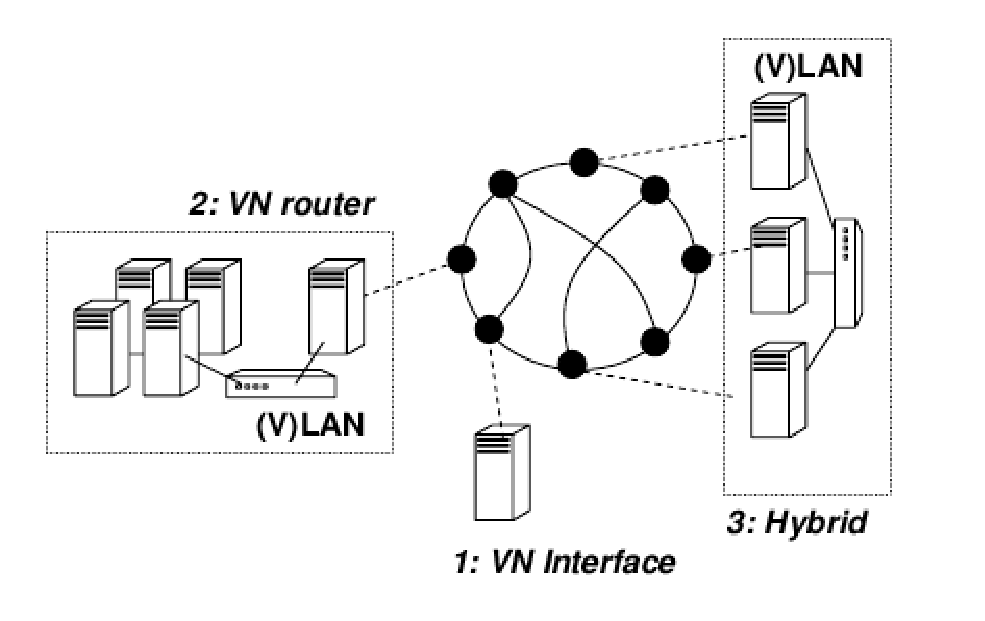
\epsfig{file=figs/three_models.png.eps}
\caption{Three VN approaches: router, interface, and hybrid}
\label{fig:three_models}
\end{figure}

This dissertation identifies methods by which a single software stack can be
implemented to support self-configuration and resource migration in a way that
is platform independent.  This method lends itself to a new architecture known
as Hybrid, allowing an instance to be run on each VPN resource but enabling
direct communication amongst peers on a LAN~\cite{sc09}.  The architectures are
shown communicating via an overlay in Figure~\ref{fig:three_models} and
compared in Table~\ref{tab:three_models}.  The two aspects that need
configuration in the local configuration beyond the VPN architecture are
address allocation, obtaining and setting an IP address on a resource, and
address resolution, determining where to route a VPN packet.  The keys to
creating this environment involve the use of standard network protocols
implemented uniformly across operating systems, including DHCP and ARP (address
resolution protocol).  Many applications make use of names instead of IP
addresses to resolve peers, as such a naming system, like DNS (domain name
service) is almost as important as address resolution and allocation.  A state
machine representation of this architecture is shown in Figure~\ref{fig:vn}.
In this representation, a VN interface is identical to a VN router with the
caveat that the TAP device is not bridged, thus isolating the VN traffic.  The
``Should Handle'' with dashed lines is a feature that is specific to the VN
hybrid; that is, a VN hybrid must be configured to communicate for a single
network device.

\begin{figure}[ht]
\centering
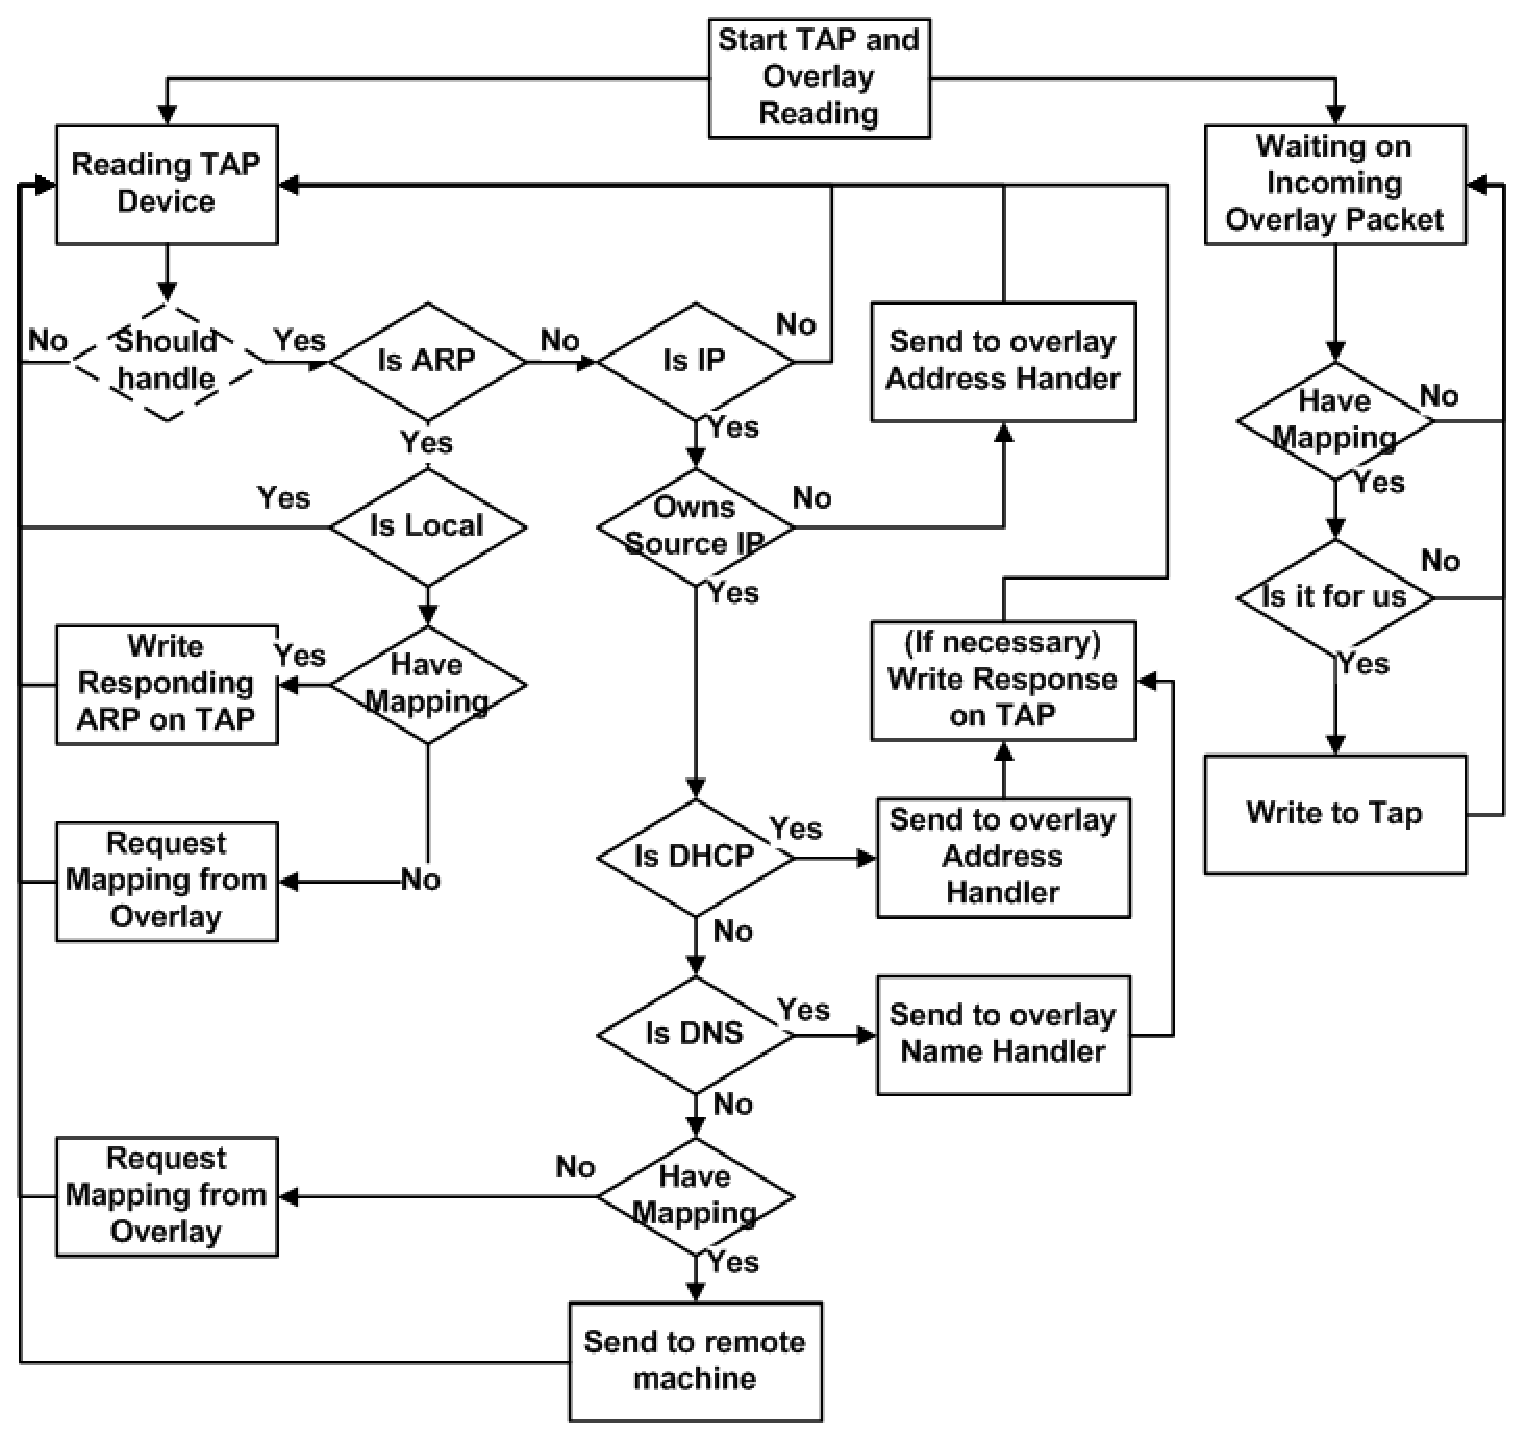
\epsfig{file=figs/vn.png.eps, width=\textwidth}
\caption{The state diagram of a self-configuring VN}
\label{fig:vn}
\end{figure}

\subsection{Local VPN Architecture}

\begin{figure}
\centering
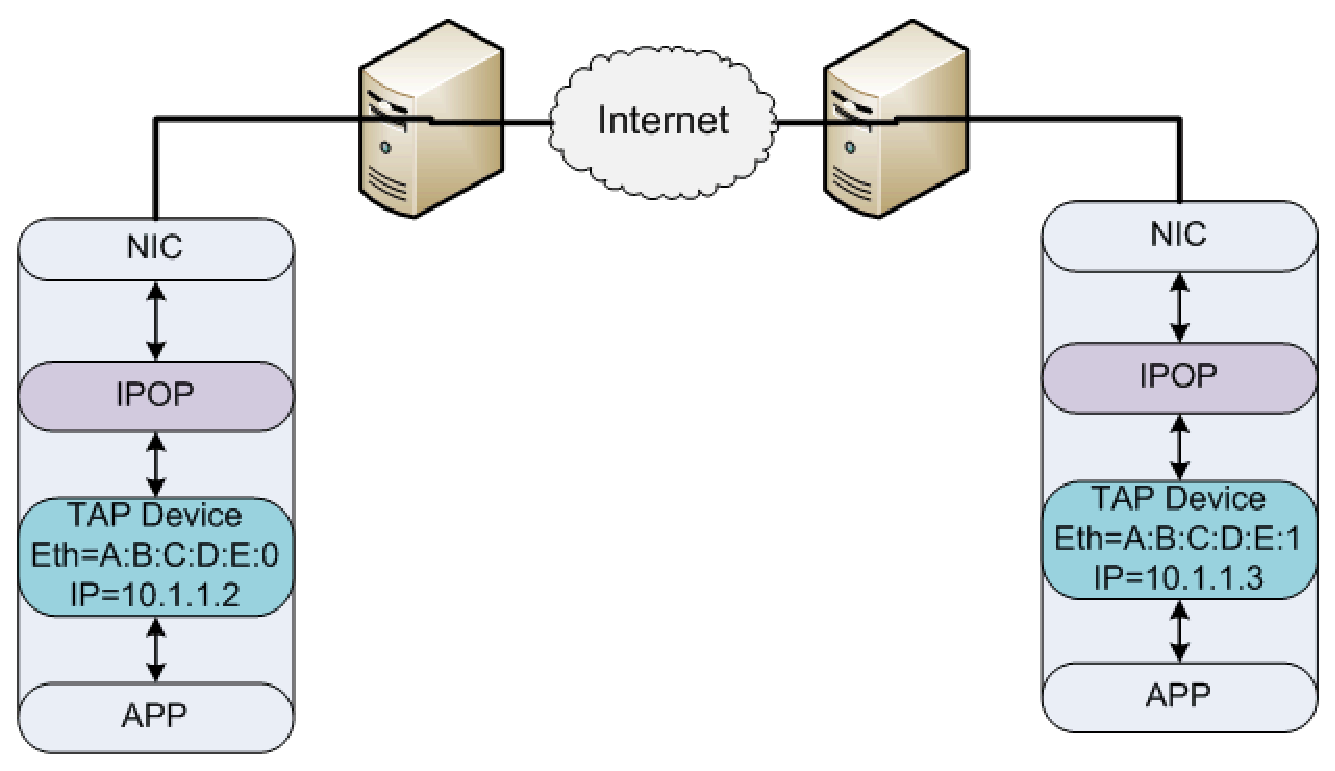
\epsfig{file=figs/tap_workstation.png.eps, width=\textwidth}
\caption{VN interface}
\label{fig:interface}
\end{figure}

As described in the introduction, the TAP device is the glue by which the local
resources communicate with the VPN.  Each approach relies on the TAP device
though in different configurations.  In the Interface
(Figure~\ref{fig:interface}), the TAP device is used directly by the user as
any other network device.  In short, packets are written to the TAP device by
the O/S (operating system) sockets and read by the VPN software to send to the
remote location, packets received by the VPN are written to the TAP device and
delivered to sockets by the O/S.  The Router (Figure~\ref{fig:router}) bridges
the TAP device to a LAN, thus packets can be routed to it and sent through the
VPN.  TAP device virtualizes a bridge to other physical networks.  

\begin{figure}
\centering
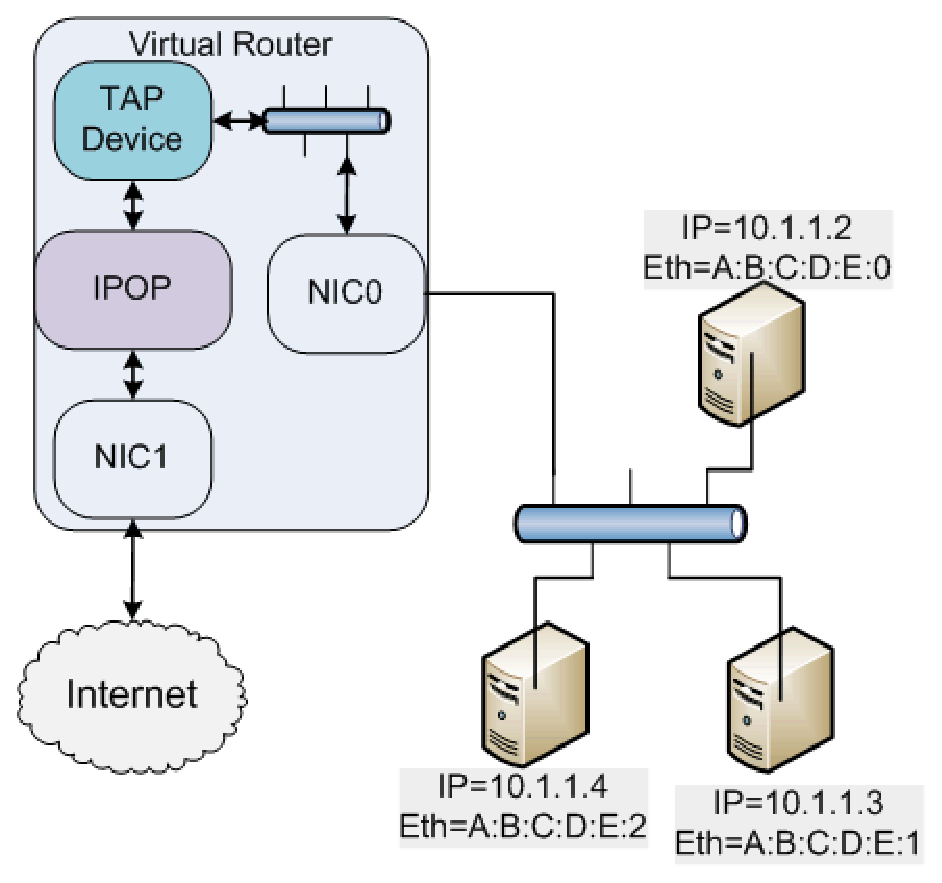
\epsfig{file=figs/tap_cluster.png.eps, width=4in}
\caption{VN router}
\label{fig:router}
\end{figure}

Finally, the Hybrid (Figure~\ref{fig:hybrid}) like the Router connects to the
LAN but only allows configuration from the local host.  In Linux this is
possible through the use of a VETH pseudo device that provides a virtual
Ethernet pair, so that one end can be bridged with the TAP device and LAN while
the other provides another interface that can be configured on the LAN, which
will be used by the VPN.  The reason for this lies in the nature of the state
of the interfaces connected to the bridge, which go into promiscuous mode, so
that all packets sent to them are forwarded on as if they are on a wire as if
there were only a single network interface.  In non-promiscuous mode, the
network card will drop packets that are not destined for that network card.  So
in that case, it is not possible to assign more than one IP address to a
bridge, because it and all devices connected to it are viewed as one big
network interface.  Connecting the VETH device allows an additional uniquely
identifiable Ethernet addresses and thus additional IP addresses.  In contrast,
aliasing a Ethernet card only provide additional IP addresses and services that
rely on layer 2 networking. In this case, some services may not work, for
example, DHCP does not work on aliased network cards.

\begin{figure}
\centering
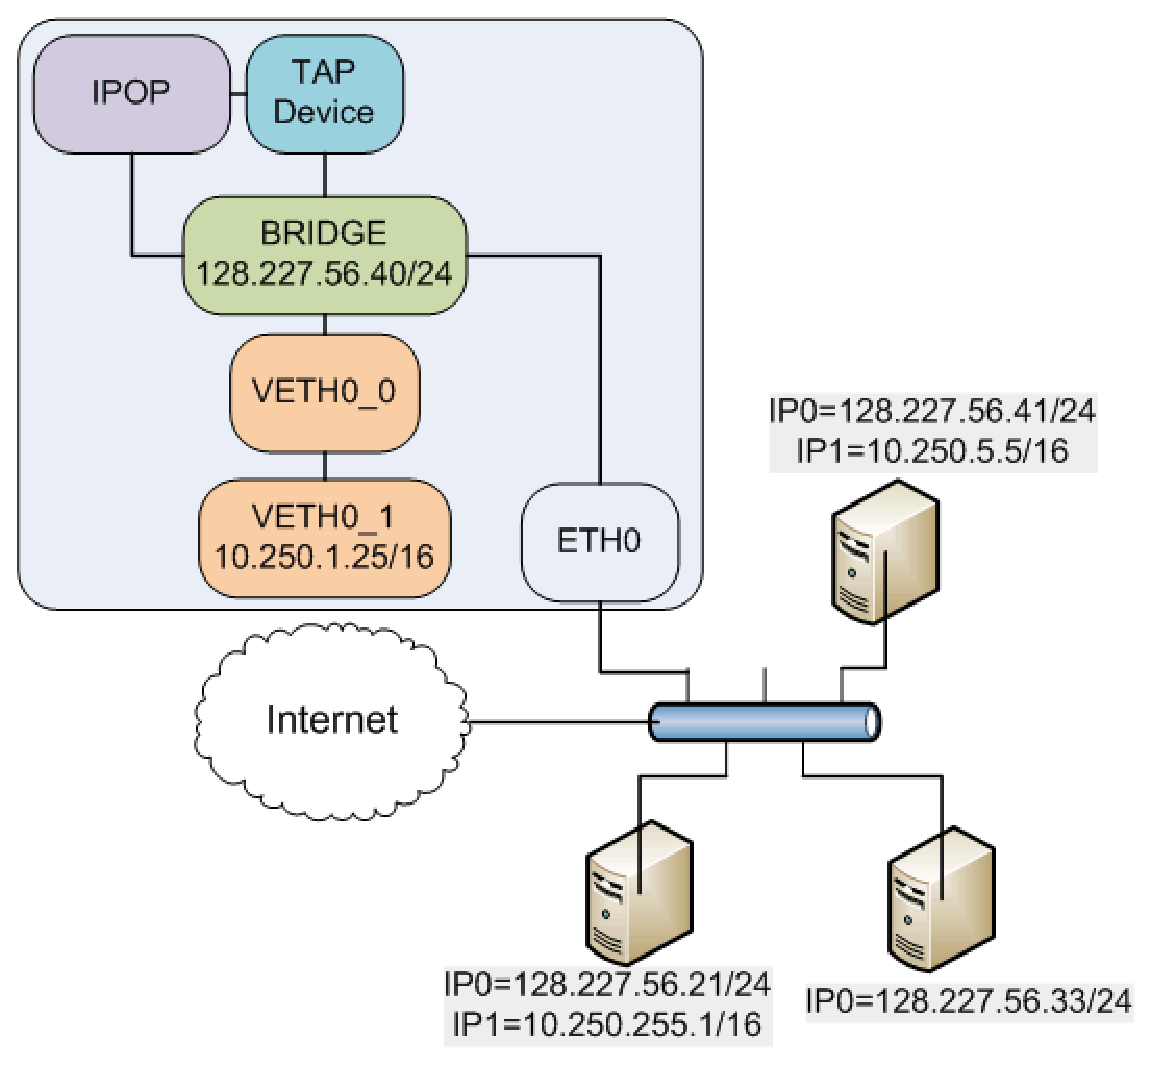
\epsfig{file=figs/tap_hybrid.png.eps, width=4in}
\caption{VN hybrid}
\label{fig:hybrid}
\end{figure}

\subsection{Address Resolution}
\label{vpns:arp}

IP is a layer 3 protocol. Layer 2 devices such as switches, bridges, and hubs
are not aware of IP addresses.  When a system wants to send a layer 3 packet
over a layer 2 network, it first uses ARP to find the layer 2 address owning
the layer 3 address.  This process, as shown in Figure~\ref{fig:arp}, begins by
the sending of a layer 2 broadcast message which contains an ARP request,
asking all members in the LAN that the node owning the target IP address
respond to the sender of the request.  If a node owns the target IP address, it
responds with an ARP reply, making themselves the sender and the original
sender is the message recipient.  The Ethernet header consists of the source
address being the sender and the target being the destination.  By listening to
these requests, layer 2 devices such as a switch can autonomously learn the
location of nodes holding Ethernet addresses are and can forward packets
through appropriate ports as opposed to broadcasting or dropping them.

\begin{figure}
\centering
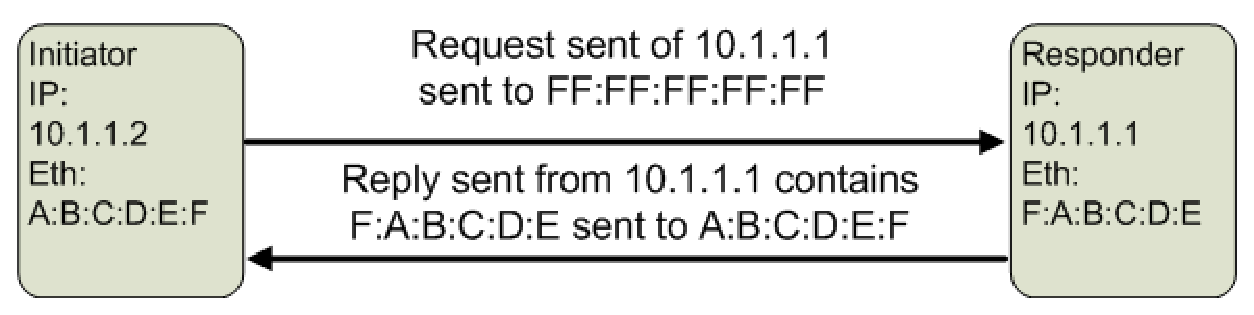
\epsfig{file=figs/arp.png.eps, width=4in}
\caption{ARP request/reply interaction}
\label{fig:arp}
\end{figure}

In a typical IP subnet, all machines talk directly with each other through
switches.  As such, they must learn each other's Ethernet address. The VN model
used herein focus on a large, flat subnet spanning across all nodes connected
to the VPN.  To accomplish this, the VN provides the ability to virtualize a
bridge, similar to proxy ARPs~\cite{RFC0925} used to implement a transparent
subnet gateway~\cite{RFC1027}.  In this scenario, the VN would need to respond
to the ARP packets with a fake layer 2 address.  Layer 2 devices in the system
would then route all packets destined for that layer 2 address to the VN.

As shown in the state machine (Figure~\ref{fig:vn}), ARPs are only responded to
if (a) they are inquiring about a VN IP address, (b) the VN address is not
locally allocated, and (c) there is a P2P:IP mapping.  If all those are true,
then an ARP response is sent back to the sender.  ARPs are occasionally sent
out during the course of communication and thus if a machine migrates to a VN
router, the VN router will no longer respond with ARPs.  An ARP response sent
by the VN requires a source Ethernet address, bridges and switches will see the
response and will forward all traffic towards the TAP device for that Ethernet
address.  A VN device can use the same Ethernet address for remote entities.

Prior to the introduction of the VN hybrid, the VNs used the Ethernet address
FE:FD:00:00:00:00 to refer to remote entities.  If each VN hybrid used this
address, there would be layer 2 collision causing a single hybrid to have all
traffic sent to it.  In hybrid mode, each VN must generate a unique ``remote''
Ethernet address at run time.  Experience and research has led to the
following solution: (1) use FE:FD for the first two bytes as they tend to be
unallocated and (2) assign random values to the 4 remaining bytes.   Applying
the birthday problem in this context, the expected probability of address
collisions is small for typical LAN environments (less than 50\% if the average
number of VN hybrid nodes on the same L2 network is 65,000). 

The key difference from the Hybrid and Router is that the Hybrid routes for only
a single node, say ``A'', and thus must ignore messages that do not originate
from ``A''.  The Hybrid model does not necessarily know about the existence of
all machines in a LAN, because it does not own them.  So when an ARP request
of some remote machine, say ``B'', is sent by ``A'', the Hybrid must send out
a matching request with the result being sent back to the pseudo-entity of the
transparent subnet gateway so that the VPN can determine if ``B'' exists
locally.  If no message is returned after a set amount of time (the reference
implementation used 2 seconds), then assuming that there is a peer in the
overlay with the IP address, the original ARP will be responded to with the
pseudo-entity being the target.

\subsection{Address Allocation}
IP addresses are traditionally allocated in one of three ways: 1) statically, 2)
dynamically through DHCP, or 3) through pseudo-random link-local addressing.
This model focuses on static and dynamic addressing.

\begin{figure}
\centering
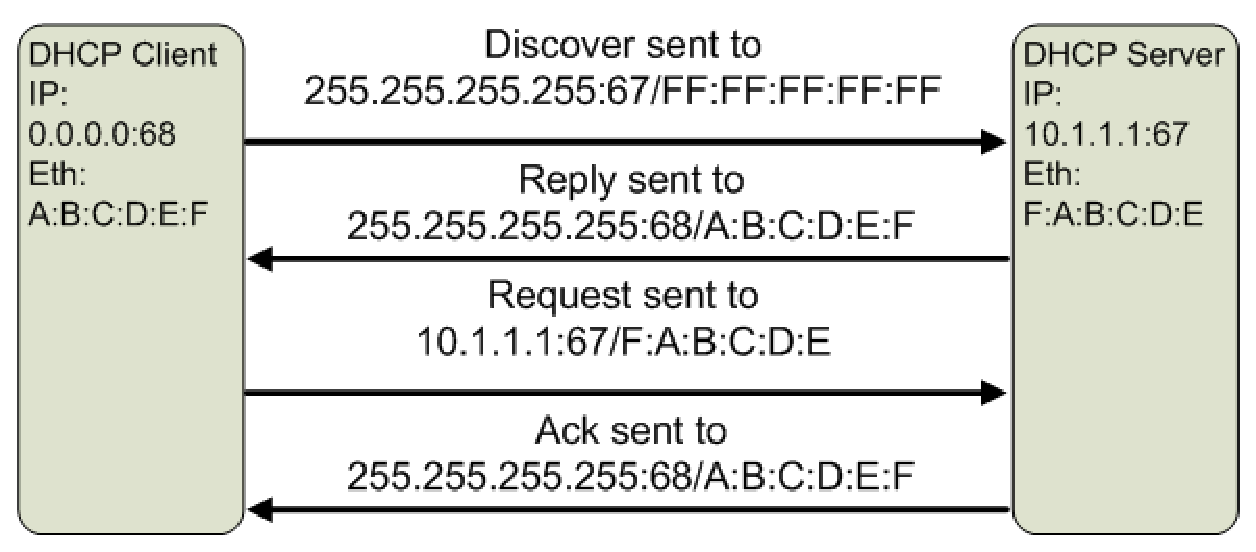
\epsfig{file=figs/dhcp.png.eps, width=4in}
\caption{DHCP client/server interaction}
\label{fig:dhcp}
\end{figure}

The network components configurable by DHCP~\cite{dhcp0,dhcp1} that are
interesting to a VPN are addresses, routing, and other networking related
features.  While many different client and servers exist, they all tend to
support the basic features of allowing the server to specify to a client and IP
address, a gateway address, and domain name servers.  As shown in
Figure~\ref{fig:dhcp}, the steps in DHCP are:

\begin{enumerate}

\item Client sends Discover packet requesting address.

\item Server receives the packet, allocates an address, and sends an Offer of
the address and other network configuration.

\item Client receives and acknowledges the Offer by sending a Request message
to accept the Offer.

\item Server receives Request message and returns an ACK message containing the
same details as the Offer.

\end{enumerate}

During the DHCP phase, the VPN communicates with a DHCP server for the VPN,
which will allocate an address for the requester.  Similarly, a VN model can
review packets coming into the VPN, review the sender IP address, and request
and notify the server of this allocation.  Treating static addresses like DHCP
enables easier configuration of the VPN, though it is difficult to handle
address conflicts.  In this model, this is done by the server ignoring the
duplicate requests, and it is up to the user to configure for a new address.
Thus DHCP provides a more reliable method in these systems.

To support scalable address allocation in decentralized systems, the
DHCP server is a virtual entity, parsing DHCP packets and interacting with
an overlay based DHT.  This approach does not need to be limited to structured
overlay based VPNs but can be introduced as an added value component.

An important aspect of DHCP is that after a machine has received an IP address
from the DHCP server, it always checks to ensure that the address has not been
allocated, as such the VPN should never respond to address resolutions for
local IP addresses.

If an overlay allocates an address to the VN, then the VN owns it.  The other
address that the VN owns is the null address, 0.0.0.0, which is sent during
DHCP to indicate that the machine has no address prior to the request.

\subsection{Domain Name Servers and Services}

Name services allow machines to be addressed with names that are more
meaningful to users than numeric addresses.  Certain applications and services
require domain name checking, such as Condor.  To support DNS, this requires
that the O/S be programmed with the VN's DNS servers IP, typically the lowest
available IP address in a subnet.  In static configuration, this process
requires the user to manually add this address, though through DHCP this is set
automatically.

In the state representation of the VN (Figure~\ref{fig:vn}), the VN checks the
IP packet to ensure that the destination IP and port match that of the virtual
DNS server and the well-known DNS port, 53.  In the event of a match, the
packet is passed to the VN's handler for domain names.  Names are typically
used for the following purposes: 1) because applications require it, and 2) to
assist users in finding resources.  To deal with 1), the DNS can
deterministically maps IP addresses to names, such as 10.250.5.5 maps to
C250005005.  2) can be solved by using the DHT and placing key:value pairs of
the form hash(namespace:hostname) to IP address and hash(namespace:IP address)
to hostname.

\section{Supporting Migration}

There has been a rapid increase in the deployment of Virtual Machines (VMs) for
use in resource consolidation in the server industry as well as the domain of
cloud computing.  Providers of cloud computing services have adopted virtual
machines as the unit of granularity for providing services and service level
agreement to the users.  Users are billed according to the number of VMs and
their uptime. Major cloud-computing providers including Amazon$^\registered$ EC2 (Elastic
Cloud 2) and Go-Grid have adopted Xen as the virtualization platform for their
services and sell compute resources in the form of virtual machines.

Apart from advantages like performance isolation, security, and portability,
one of the significant advantages of using VMs is the capability to migrate the
VM with its entire software stack from one physical host to another.  This
migration may be performed in a stop-restart manner, where the VM is paused,
migrated to another host and restarted, or in a live mode, which attempts to
minimize down time to reduce interruption of services running on the VM.

VMs including Xen~\cite{xen-live}, VMware ESX~\cite{vmotion} and KVM~\cite{kvm}
support migration with two critical requirements: (1) file systems (disk
images) must be on a shared storage system (i.e. network file systems or
storage area networks) and (2) to maintain network connectivity, the migration
must occur within an IP subnet.  In order to retain network connectivity after
migration, the VMM (virtual machine manager) must notify the LAN of the VM's
new location.  The new VMM host generates an unsolicited ARP reply which
broadcasts to the entire network the VM's new location.  

The VN Interface and Hybrid models support migration of the virtual address
using techniques previously described by Ganguly et al.~\cite{ipop}.  This is a
product of the decentralized, isolated overlay approach where each overlay end
point has a one-to-one mapping to VN end point, e.g., P2P to IP.  When a VN
Interface or Hybrid model migrates, the overlay software must reconnect to the
overlay, at which point, packets will begin to be routed to the VN endpoint
again, completing migration.

Unlike Interface and Hybrid models, the VN Router does not support a one-to-one
mapping.  In fact, a VN router tends to have one P2P address for many IP
addresses.  When a machine with a VN IP wants to migrate, it cannot also take
its P2P address with it otherwise it would end connectivity for the rest of the
members of the VN router shared  overlay end point.  A solution to this
problems requires the ability to delete IP-to-P2P mappings in the DHT, detect
new addresses on the network, and inform senders that an IP is no longer
located at that overlay end point.  With these capabilities, transparent
migration can be achieved for the VN router model as follows. 

The VMM initiates a migration on a source node. Until the migration completes,
the VN router at the source continues to route virtual IP packets for the VM.
Upon completion of migration, the VN router at the target learns about the
presence of the migrated VM by either receipt of an unsolicited ARP or by
proactively issuing periodic broadcast ICMP (Internet Control Message Protocol)
messages on its LAN.  The VN router attempts to store (Put) the IP:P2P address
mapping in the DHT, and queries for the existence of other IP:P2P mapping(s).
If no previous mappings are found, the VN router assumes responsibility for the
IP address. Otherwise, the VN router sends a migration request to each P2P
address returned by the DHT. The VN router receiving a migration request
confirms the existence of the IP address in its routing table and that if there
is that there is no response to ARP requests sent to the IP address.  If these
conditions hold, it deletes its IP:P2P mapping from the DHT and returns true to
the migration request; otherwise, it returns false. If the migration request
returns true, the VN router at the target LAN starts routing for the virtual IP
address; if it returns, false, the VN router does not route for the virtual IP
address until the previous IP:P2P mapping expires from the DHT.

In addition to VN routers synchronizing ownership of the migrated virtual IP
address, any host that is connected to that machine must be informed of the new
P2P host.  Over time, this will happen naturally as ARP cache entries expire
and the IP:P2P mapping is looked up from the DHT.  Additionally, the VN router
at the source may keep forwarding rules for the migrated IP address for a
certain period of time, akin to mobile IP but not on a permanent basis.  A more
direct approach, as implemented in the prototype, involves the VN router
notifying the connected host of a change in ownership, resulting in the host
querying the DHT for the updated P2P end point.  An evaluation of trade offs in
the migration design, while interesting, is outside the scope of this
dissertation. 

A static address allocation is similar to a migration without there being an
IP:P2P value in the DHT, though without querying the DHT, the situation is
unclear.  Systems that use DHCP only must have some method for detecting new
addresses, because there is no guarantee that a DHCP will occur immediately
following migration, in fact, depending on the lease time that is highly
unlikely.  Using an insecure DHT that supports deletes is sketchy as it would
be relatively easy for machines to perform man in the middle attacks by
deleting keys which they do not own.  Even the use of passwords mentioned in
DHT literature is not sufficient as it is not immune to collusion, or Sybil,
attacks.

VN router migration was analyzed through the use of two Xen-based VMware VMs
co-located on the same quad-core Xeon 5335 2 GHz machine each with 1 GB memory
allocated using a minimally configured O/S with a SSH (secure shell) server.
The evaluation attempts to understand overlay overheads of the approach.  The
experiment, as shown in Figure~\ref{fig:migration_ring}, involved migrating a
Xen guest VM between two Xen host VMMs running in VMware.  Although they are
hosted in the same infrastructure, the two domains are connected to two
separate VLANs, and thus isolated.  The resource information is stored in a DHT
running on top of PlanetLab.  Thus the migration overheads in the experiment
capture the cost of wide-area messaging in a realistic environment.  During the
course of the experiment, over 50 different IP addresses were migrated 10 times
each in an attempt to gain some insights in the cost of using the DHT with
support for deletes and VN router messages as a means to implement migration.
The result, presented in Figure~\ref{fig:mig} gathered from the experiment was
how long the VN IP was offline, measured by means of ICMP ping packets.  On
average, the overhead of VN migration was 20 seconds. This overhead is in
addition to the time taken to migrate a VM, since the VN routers begin to
communicate only after migration finishes. 

\begin{figure}
\centering
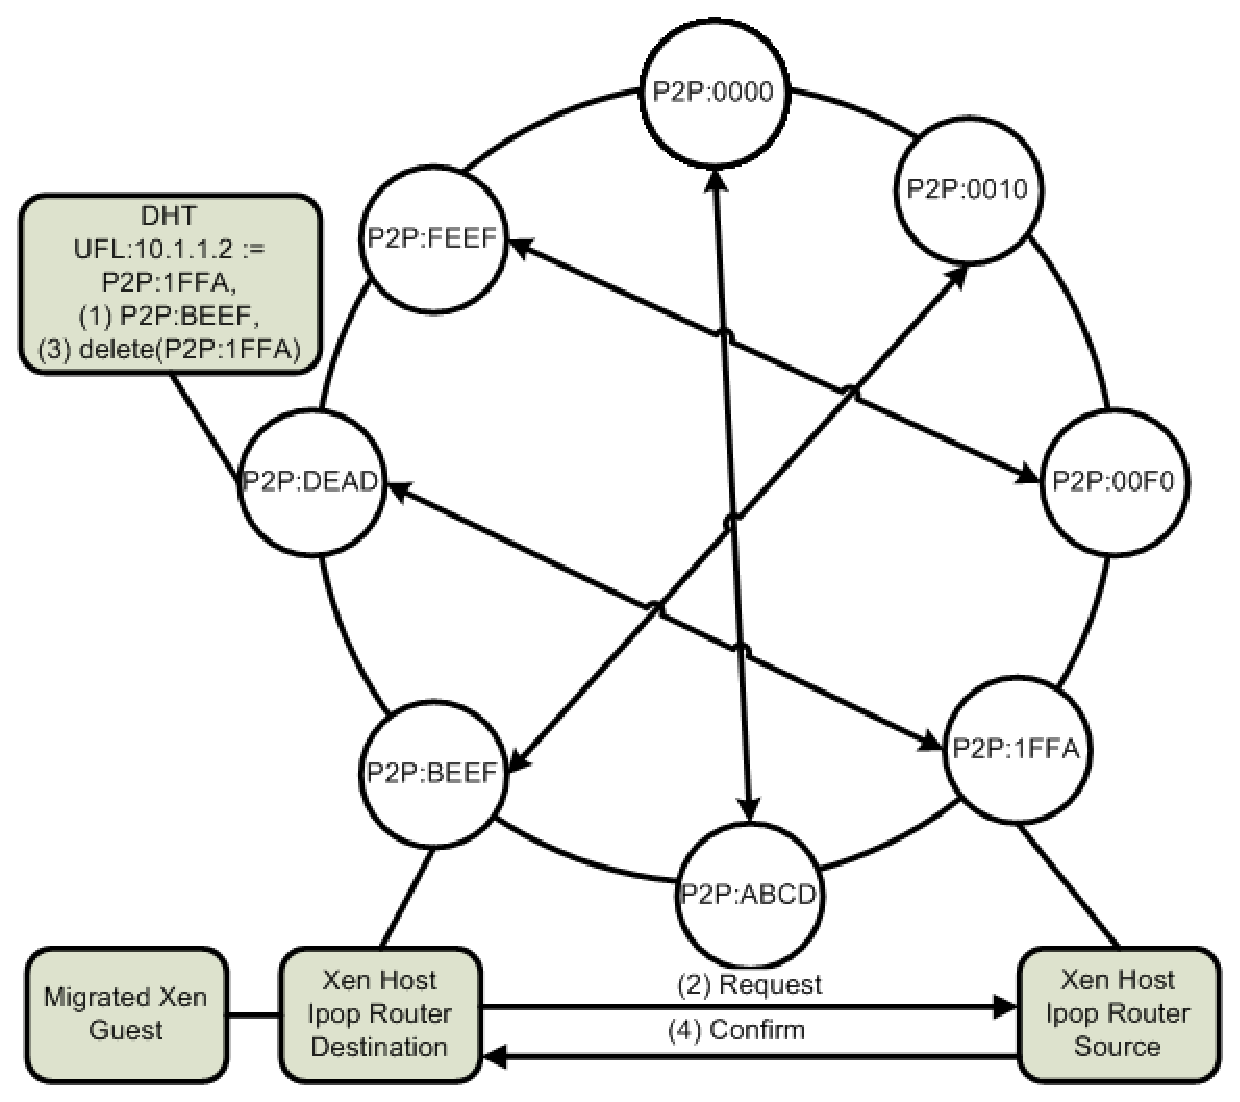
\epsfig{file=figs/Migration.png.eps, width=\textwidth}
\caption{VN router migration}
\label{fig:migration_ring}
\end{figure}

\begin{figure}
\centering
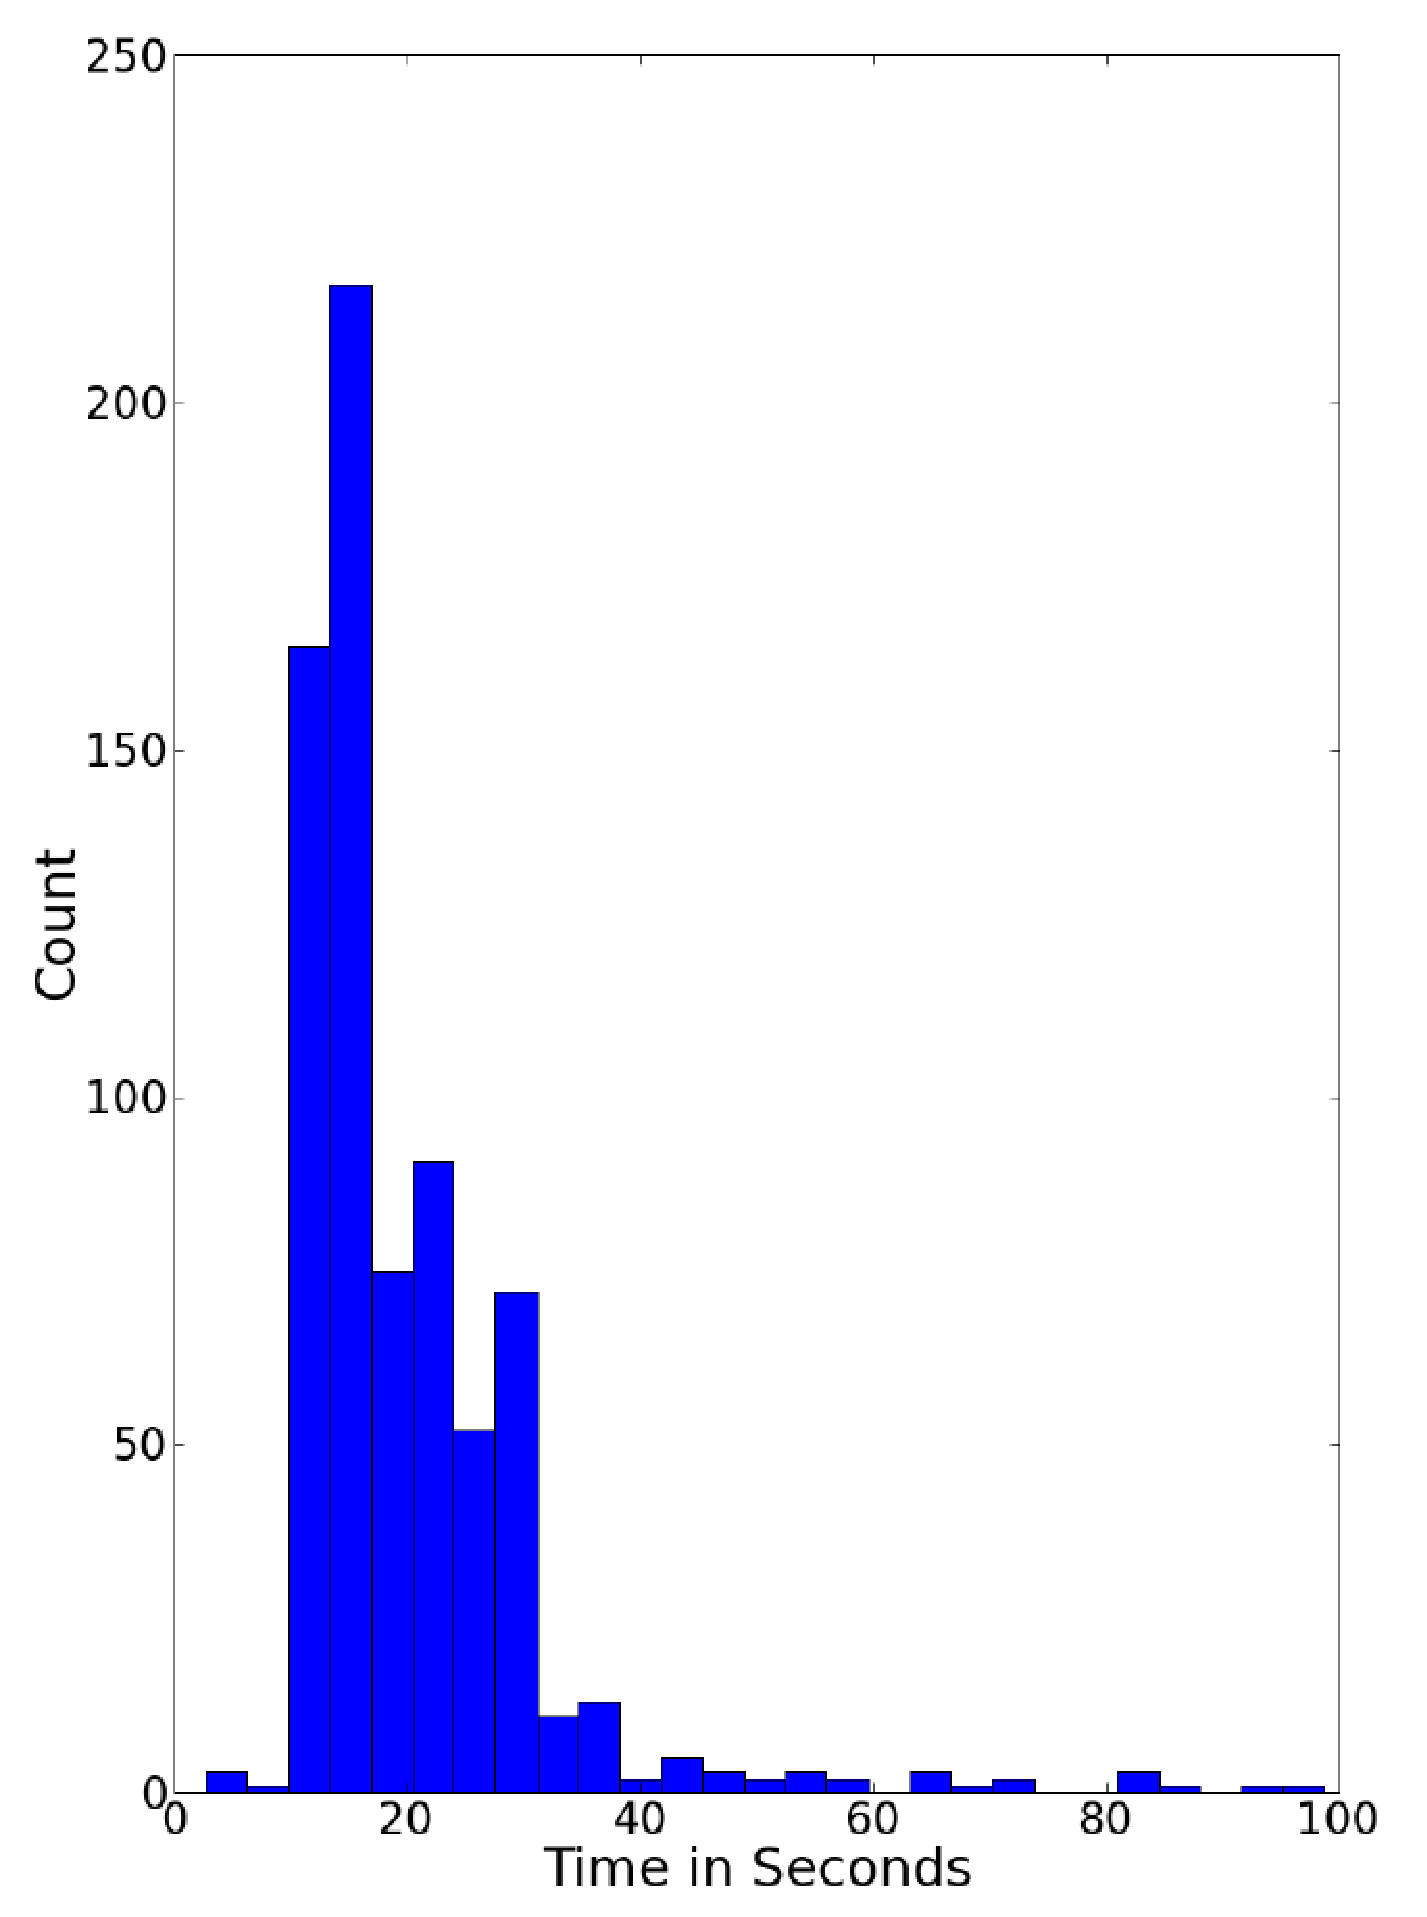
\epsfig{file=figs/migration_results.png.eps, width=3.5in}
\caption{VN router migration evaluation}
\label{fig:mig}
\end{figure}

\section{Evaluation of VPN Network Configuration}

This experiments explores bandwidth and latency in a distributed VPN system to
motivate the usage of P2P links in a VPN.  The VPNs used are include the
prototype, which extends from IPOP; OpenVPN$^\registered$; and Hamachi$^\registered$.  OpenVPN$^\registered$ represents a
typical centralized VPN, while Hamachi$^\registered$ represents a well-tuned P2P-link VPN.
The evaluation was performed on Amazon$^\registered$ EC2 using small instance sized Ubuntu
i386 instances to create various sized networks ranging from 1 to 32.  OpenVPN$^\registered$
uses an additional node as the central server and Hamachi$^\registered$ has an upper bound of
16 due to limitations in the Linux version at the time of this evaluation.  To
perform bandwidth tests, the instances are booted and query an NFS for the list
virtual IP addresses, peers are ordered such that half the peers are act as
clients and the other half the peers creating a 1 to 1 mapping between all
sets.  Latency and bandwidth tests are performed using netperf's request-reply
and streaming tests respectively.  Prior to the start of the tests, peers have
no knowledge of each other, except the virtual IP addresses, thus connection
startup costs are included in the test.  Test are run for 10 minutes diluting
the connection initiation overhead but represent an example of real usage.
Results from the clients are polled at all locations and averaged together,
though the OpenVPN$^\registered$ server is measured separately.  IPOP and OpenVPN$^\registered$ use
authenticated 128-bit AES, while Hamachi$^\registered$ does not allow configuration of the
security parameters and uses the default Hamachi$^\registered$ settings.

\begin{figure}
\centering
\epsfig{file=figs/latency.eps}
\caption{System transaction rate for various VPN approaches}
\label{fig:latency}
\end{figure}

Figure \ref{fig:latency} and \ref{fig:bandwidth} present the results for latency
and bandwidth respectively.  Latency is measured in transactions of successful
request/reply messages.  In the latency test, it is obvious that having the
central server increases the delay between the client and server and the results
degrade more quickly as additional peers are added to the system.  In small
systems, OpenVPN$^\registered$ shines probably due to optimized software, though as the system
grows, the system bandwidth does not.  By the time 8 peers have entered into
the system, both decentralized approaches perform better than the OpenVPN$^\registered$
solution.  To summarize, decentralized VPN approaches provide better
scalability, which can be immediately noticed by low latency times and, as the
system grows, available bandwidth.

\begin{figure}
\centering
\epsfig{file=figs/bandwidth.eps}
\caption{System bandwidth for various VPN approaches}
\label{fig:bandwidth}
\end{figure}

\section{Evaluation of VPN Local Configuration}

This section presents an evaluation of the different VN models, using prototype
implementations built upon IPOP.  The grid evaluation simulates a client/server
environment and investigate CPU / networking overheads related with each
approach.  In addition a cloud deployment shows a proof of concept that
connects multiple cloud and local resources as well as evaluation of overhead
of the different approaches in WAN and LAN environments.  In all WAN
experiments, a wide-area IPOP overlay network with approximately 500 overlay
nodes distributed across the world on PlanetLab resources is used to bootstrap
VN connections and to support DHT-based storage and P2P messaging.

The proposed VN models place varying demands on the resources of the systems
involved. The evaluation focuses on CPU as experience suggest that this is the
most significant limiting factor.  As will be presented, the CPU load offered
by these models depends on the bandwidth of the underlying network link, since
a larger bandwidth requires more processing of packets.  The tools for
evaluating these VN models are Netperf and SPECjbb$^\registered$.

Netperf~\cite{netperf} is used to estimate the latency and bandwidth of the
different VN models. The latency is measured by deploying Netperf in the
TCP\_RR mode, which measures the number of 1-byte request-receive transactions
that can be completed in a second. The bandwidth is estimated by running Netperf
in the TCP\_STREAM mode, which is a bulk transfer mode. It should be noted that
in situations where the link bandwidths were asymmetric, Netperf is deployed in
both directions.  Since both latency and bandwidth are dependent on the CPU
comparison, evaluations that include CPU utilization tasks require creating
a baseline first where only Netperf is the only active workload.

SPECjbb$^\registered$~\cite{specjbb} simulates a three-tier web application with all the
clients, the middle tier, and the database running on a single system in a
single address space (inside a Java virtual machine). On completion, the
benchmark provides the metric in terms of business of operations per second
(bops). The bops score of the system under test depends on both the CPU and the
memory in the system, as the entire database for the benchmark is held in
memory. This benchmark generates negligible disk activity and no network
activity. 

\subsection{On the Grid}

The initial evaluation involves testing a client-server environment.  The
baseline hardware consisted of quad-core 2.3GHz 5140 Xeon with 5 GB memory and
Gigabit network connectivity.  Each VM was allocated 512 MB of RAM and ran
Debian 4.0 using a Linux 2.6.25 kernel.  The client side consisted of 4 VMs on
5 machines.  The server side consisted of 5 VMs on one machine with 4 acting as
servers and 1 acting as a gateway, which was necessary to control bandwidth
into the system, done through the Linux utility tc~\cite{tc}, traffic control.
In this environment, each server had 5 clients communicating with it.  The
setup is shown in Figure~\ref{fig:gridsetup}.  The VM ``Servers'' ran
SPECjbb$^\registered$ and were also the site for the collection of the netperf
benchmarks.  All the VM ``Servers'' were connected through the TC Gateway
through host-only networking to the VM ``Clients''.  All traffic for the VM
``Servers'' passes through the TC Gateway, which also doubled as the Router in
the Router experiments.

\begin{figure}
\centering
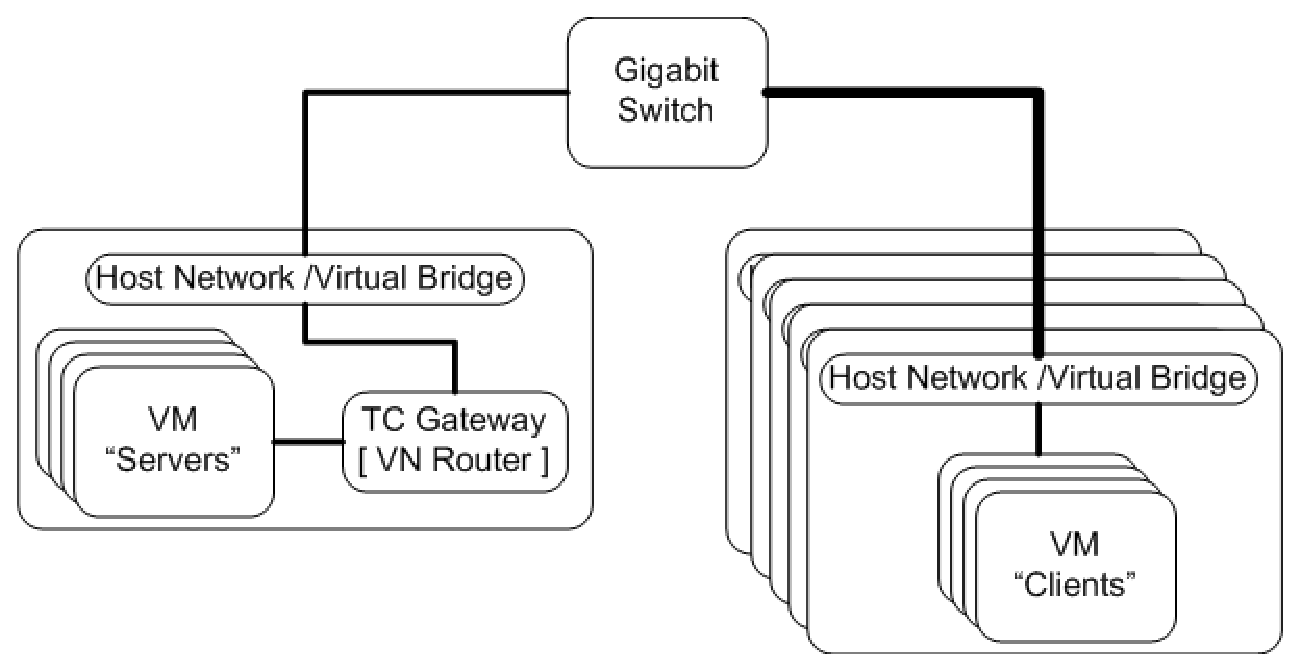
\epsfig{file=figs/grid_setup.png.eps, width=4in}
\caption{Grid evaluation setup}
\label{fig:gridsetup}
\end{figure}

All the evaluations presented in Figures \ref{fig:stream.netperf},
\ref{fig:rr.netperf}, \ref{fig:stream.spec}, and \ref{fig:rr.spec} are marked
up in the same fashion.  The evaluations were performed with and without a
SPECjbb$^\registered$ load.  Lines are of the form (no spec, spec).(phys,
interface, router).  Where ``spec'' indicates SPECjbb$^\registered$ benchmark
is active, while ``no spec'' indicates that SPECJbb is inactive. ``phys''
implies the absence of IPOP with benchmarks occurring directly over the
``physical'' network card.  ``interface'' and ``router'' present the results
for VN interface and Router respectively.

The maximum bandwidth of 600 Mbps is achieved when neither virtual network nor
traffic shaping are enabled (``no spec.phys'' at 1000 Mbps limit in
Figure~\ref{fig:stream.netperf}), which is only 60\% of the theoretical
maximum.  This limit is most likely the cost of VMMs, specifically the time
required for a packet to traverse both VMMs networking stack as well as the
hosts networking stack.  Another observation was that transactions per second
(Figure~\ref{fig:rr.spec}) do not improve significantly for \textbf{tc}
bandwidth limit above 25 Mbps in all cases; thus focus is on only the relevant
data up to this limit.

\begin{figure}
\centering
\includegraphics[width=4in]{figs/stream.netperf.jpg.eps}
\caption{Grid Netperf bandwidth (TCP STREAM) evaluation}
\label{fig:stream.netperf}
\end{figure}

\begin{figure}
\centering
\includegraphics[width=4in]{figs/rr.netperf.jpg.eps}
\caption{Grid Netperf latency (TCP RR) evaluation}
\label{fig:rr.netperf}
\end{figure}


Distinguishing features of the different VN models include the following.
Figure~\ref{fig:stream.netperf} shows that bandwidth in all VN models is
comparable with traffic control limit up to 75 Mbps. Beyond this point, the
interface model achieves better bandwidth than the Router (VN processing
is distributed across multiple processes); the spec/no spec ratio in the router
model is smaller than in the interface model because there is less resource
contention caused by VN processing on end nodes. For the same reason, the
Router tends to achieve better SPEC results (Figure~\ref{fig:stream.spec}) than
the interface.  Figure~\ref{fig:rr.netperf} shows that the Router performs
poorly compared to the interface model in terms of transactions/second, though
it achieves a better ratio of SPECjbb$^\registered$ score (Figure~\ref{fig:rr.spec}) to
transactions than the interface at constrained bandwidths (less than 5 Mbps).

\begin{figure}
\centering
\includegraphics[width=4in]{figs/stream.spec.jpg.eps}
\caption{Grid SPECjbb evaluation with Netperf TCP STREAM load}
\label{fig:stream.spec}
\end{figure}


\begin{figure}
\centering
\includegraphics[width=4in]{figs/rr.spec.jpg.eps}
\caption{Grid SPECjbb evaluation with Netperf TCP RR load}
\label{fig:rr.spec}
\end{figure}

The hybrid method was tested, and results were nearly identical to those of the
interface, from the point of view of the WAN part of the VN, it is the same
architecture.  These results are not reported in the plots as they add little
value and further obfuscate the results.

The bandwidth cap observed in the Router approach reflects the performance
achieved by the current prototype of the router, subject to VM overheads. The
use of VM is an assumption that is valid in the domain of cloud computing where
all resources run in a VM. This experiment focused on the interplay between
resource consumption by overlay routers and application performance.  Optimized
user-level overlay routers running on dedicated physical machines have been
reported to achieve performance near Gbit/s in related work~\cite{vine2}.

One thing that left unevaluated that may provide more interesting data would be
providing the VN router dedicated hardware.  In the test environments, this was
infeasible, because all but one of the machines in the lab run VMware Server 1,
which has a bug with setting the virtual network card in promiscuous mode.
This effectively makes it impossible for a VM to be a VN router as no packets
will ever make their way into the VM, as the VMM will reject all packets.  As
such, the machines hosting the servers had VMware Server 2, which does allow
setting a network interface into promiscuous mode.

\subsection{In the Clouds}

The goal of this experiment is to demonstrate the feasibility of connecting
multiple cloud providers as well as local resources together through virtual
networking.  The sites chosen for evaluation were local resources at University
of Florida and cloud resources provided by Amazon$^\registered$ EC2 and GoGrid$^\registered$.  A
qualitative observation here was that the differences in the networking
infrastructure exposed by different cloud providers reinforce the importance of
the virtual network to allow flexibility in how end nodes are connected.
Specific network configurations for the clouds were as follows:

\begin{itemize}

\item Amazon$^\registered$ EC2 provides static IP networking (public and private), no
Ethernet connectivity, and no ability to reconfigure IP addresses for network.
Currently, only the VN interface model is supported.

\item GoGrid$^\registered$ provides 3 interfaces (one public, statically configured, and two
private, which can be configured in any manner); the 2 private interfaces are
on separate VLANs supporting Ethernet connectivity. The VN interface, router,
and hybrid models are supported.

\end{itemize}

This experiment narrows down the performance evaluation to focus on WAN and LAN
performance of VNs in cloud environments and consider Netperf single
client-server interactions only. Amazon$^\registered$ only supports Interface mode, thus it
is only evaluated in the WAN experiment. It has been observed that, within
Amazon$^\registered$, the VN is able to self-organize direct overlay connections~\cite{wow}.
Each test was run 5 times for 30 seconds, the standard deviation for all
results was less than 1.  Because of this, only the average is presented in
Table~\ref{tab:cloud-wan}.

\begin{center}
\begin{table}
\caption{WAN results for inter-cloud networking}
\begin{tabular*}{\textwidth}{@{\extracolsep{\fill}}
l
S[table-format=2.2,table-number-alignment=right]
S[table-format=2.2,table-number-alignment=right]
S[table-format=2.2,table-number-alignment=right]
@{}
}

\hline & 
\multicolumn{1}{c}{EC2 / UF} &
\multicolumn{1}{c}{EC2 / GoGrid$^\registered$} &
\multicolumn{1}{c}{UF / GoGrid$^\registered$} \\ \hline

Stream Phys (Mbs) & 89.21 & 35.93 & 30.17\\
Stream VN (Mbs) & 75.31 & 19.21 & 25.65\\
RR Phys (Trans. / s) & 13.35 & 11.09  & 9.97 \\
RR VN (Trans. / s) & 13.33 & 10.69 & 9.76 \\ \hline

\end{tabular*}
\label{tab:cloud-wan}
\end{table}
\end{center}

It can be seen in Table~\ref{tab:cloud-wan} that the VN adds little overhead in
the Netperf-RR experiment. Between UF and GoGrid$^\registered$ as well as between UF and
Amazon$^\registered$ EC2, the overhead for the Stream experiment was about 15\%.  This may be
attributed to the additional per-packet overhead of the VN and the small MTU
set for the VN interface (1200).  The MTU, or maximum transmission unit, is the
largest packet that is sent from an interface.  IPOP conservatively limits the
VN MTU to 1200 down from the default 1500 to allow for overlay headers and to
work properly with poorly configured routers, which has encountered in
practical deployments.  A more dynamic MTU, which will improve performance, is
left as future work.  The EC2 / GoGrid$^\registered$ experiment had greater overhead which
could possibly be attributed to by the VM encapsulation of cloud resources.

Table~\ref{tab:cloud-lan} shows that some of the performance expectations for
the different models in a LAN were accurately predicted while others were not
so clear.  Stream results match the expectation that VN models hybrid and
router bypass virtualization and get near physical speeds, whereas interface
does not.  Interestingly, RR had rather poor results for Router and Hybrid
though further testing seems to indicate that this is an issue of using the
VLAN connected network interfaces as opposed to the public network connected
interface.

\begin{center}
\begin{table}
\caption{LAN results performed at GoGrid}
\begin{tabular*}{\textwidth}{@{\extracolsep{\fill}}
l
S[table-format=4.0,table-number-alignment=right]
S[table-format=4.0,table-number-alignment=right]
S[table-format=4.0,table-number-alignment=right]
S[table-format=4.0,table-number-alignment=right]
@{}
}

\hline & 
\multicolumn{1}{c}{VN Interface} &
\multicolumn{1}{c}{VN Router} &
\multicolumn{1}{c}{VN Hybrid} &
\multicolumn{1}{c}{Physical} \\ \hline
Stream (Mbs) & 109 & 325 & 324 & 327 \\
RR (Trans. / s) & 1863 & 2277 & 2253 & 3121 \\ \hline
\end{tabular*}
\label{tab:cloud-lan}
\end{table}
\end{center}

\begin{center}
\singlespacing{
\footnotesize{
\begin{longtable}{p{.8in}p{1.15in}p{1.3in}p{1.25in}p{1.25in}}
\caption{Virtual network comparison} \\

\hline & Overlay & Routing & Configuration & Miscellaneous \\ \hline
\endfirsthead

\multicolumn{5}{l}{\normalsize{Table \ref{tab:virtual_networks}. Continued}}\\
\hline & Overlay & Routing & Configuration & Miscellaneous \\ \hline
\endhead

IPOP
&
%Overlay
Structured P2P overlay with $\log(N)$ routing hops, where N is the size of P2P
network. Self-optimizing shortcuts and STUN-based NAT traversal.
&
%Routing
Mapping stored in DHT resolves virtual IP address to P2P address. Virtual
network packets are routed to corresponding P2P address.
&
%Configuration
Each machine runs P2P VPN software with a dynamic IP address in a common subnet.
Common configuration shared amongst all hosts.
&
% Misc.
Supports encrypted P2P links and end-to-end VPN tunnels (unpublished work).
Migration possible; routes self-configure without user intervention, product of
the P2P overlay.
\\
N2N
&
%Overlay
Unstructured P2P network, super nodes provide control paths, forms direct
connections for data.
&
%Routing
Broadcast for discovery and overlay for control.  No organization, no guarantees
about routing time.
&
%Configuration
Requires N2N software at each host, must connect to a super node.  Supports
layer 2 Ethernet network.
&
% Misc.
Supports shared secrets to create private tunnels between edges.  Migration not
discussed, but potentially free due to layer 2 approach.
\\
OCALA
&
%Overlay
Not tied to any specific overlay, layer 3 middleware.
&
%Routing
Based upon chosen overlay.
&
%Configuration
Requires OCALA stack, overlay configuration, and IP to overlay mapping.
&
% Misc.
Security is overlay based or SSH tunnels.  Migration not mentioned.
\\
SoftUDC VNET
&
%Overlay
Decentralized with explicitly configured overlay routes.
&
%Routing
Broadcast for discovery.
&
%Configuration
Requires software on each host and one proxy per site.  Layer 2 networking.
&
%Misc.
Security is not discussed nor is wide-area migration.
\\
ViNe
&
%Overlay
ViNe authority configures global network descriptor table (GNDT) explicitly at
each router. Supports proxying to one location through another and NAT traversal.
&
%Routing
GNDT provides overlay routes for all routers in overlay.
&
%Configuration
Each subnet is allocated a single router.  Each host must be configured for
regular and ViNe networks, but no VN software needed on host.
&
% Misc.
Supports encrypted tunnels between ViNe routers, migration not discussed.
\\
Violin
&
%Overlay
Decentralized network with statically configured overlay routes.
&
%Routing
Broadcast discovery for Ethernet, static routes for IP subnet.
&
%Configuration
Virtual hosts connect VMs to the VN.  Hosts connect to virtual switches or
proxies (gateways).  Switches connect to proxies.  Sites are typically
allocated an IP address space.
&
% Misc.
Security potentially through the use of SSH Tunnels.  Migration possible;
requires reconfiguration of switches. 
\\
Virtuoso VNET
&
%Overlay
Decentralized with explicitly configured overlay routes.
&
%Routing
Broadcast for discovery.  Bridging learns paths after initial discovery.  Virtual
network packets are routed between VNET proxies.  Can be configured manually.
&
%Configuration
Each site runs a proxy providing Ethernet bridge to other proxies.  VM hosts
forward packets to local proxy.  Proxies configured to connect to other proxies.
&
% Misc.
Security through the use of SSL and SSH Tunnels.  Layer 3 migration, product of
layer 2 virtualization.
\\
OpenVPN$^\registered$
&
%Overlay
Centralized
&
%Routing
Central server
&
%Configuration
Servers manually configured to connect with each other.  Clients randomly select
server from pre-shared list
&
%Misc
All communication traverses central server, end to end traffic by default is not
protected from central server
\\
Tinc and CloudVPN
&
%Overlay
Decentralized with explicitly configured overlay routes
&
%Routing
Broadcast for discovery, messages traverse overlay
&
%Configuration
Manual configuration
&
%Misc
NAT traversal through relays only
\\
Hamachi$^\registered$
&
%Overlay
Centralized Discovery, P2P links
&
%Routing
Peers establish security links and end point information from a central
server, attempt to form direct connections, if fails, relay through central
server
&
%Configuration
Select a network to join or create and specify a password, communicates with a
centralized server to manage the VPN
&
%Misc
Lacks portability, Linux version out of date, inability to run external relay
servers, UDP NAT traversal
\\
GBridge
&
%Overlay
Centralized Discovery, P2P links
&
%Routing
Peers establish security links and end point information from a central
server, attempt to form direct connections, if fails, relay through central
server
&
%Configuration
Select a network to join or create and specify a password, communicates with a
centralized server to manage the VPN
&
%Misc
Lacks portability and inability to run external relay servers, uses TCP NAT
traversal
\\
Wippien
&
%Overlay
Centralized Discovery, P2P links
&
%Routing
Peers discover and authenticate each other through XMPP chat server, security
provided unknown, peers attempt to form direct connections with each other, if
that fails, no communication
&
%Configuration
All peers must be members of associated XMPP chat rooms and be connected to the
chat
&
Requires a GUI, difficulty penetrating NATs, claims to be open source though
most of the code is unavailable, Linux client out of date and does not support
NAT traversal
%Misc
\\
P2PVPN
&
%Overlay
Centralized Discovery, P2P links
&
%Routing
Peers discover each other through a BitTorrent$^\registered$ tracker and attempt to form
direct links with each other, attempts to form all-to-all connectivity, if
direct links are unavailable, indirect links can be used to forward packets
&
%Configuration
Peers must join the same tracker and use common shared secret
&
%Misc
Work in progress to make more unstructured, currently a cross between
centralized and decentralized
\\ \hline
\label{tab:virtual_networks}
\end{longtable} } }
\end{center}
